\section{Výsledky operátorov mapovania tónov}

Testované scény boli hodnotené a porovnávané pri použití rôzných nastavení pre štyri operátory mapovania tónov.
Globálne operátory \texttt{Reinhard} a \texttt{Drago} neumožňujú na scéne s vysokým dynamickým rozsahom získať uspokojivý
výsledok, kde by boli jasne viditeľné zároveň tmavé a svetlé oblasti. Na prvých dvoch obrázkoch \ref{fig:reinhards}
máme dobre viditeľnú svetlú časť scény, no keď chceme pridať jas aj na tmavej časti, svetlá časť sa preexponuje
(tretí obrázok).

\begin{figure}[h!]
  \centering
  \begin{subfigure}{0.3\textwidth}
      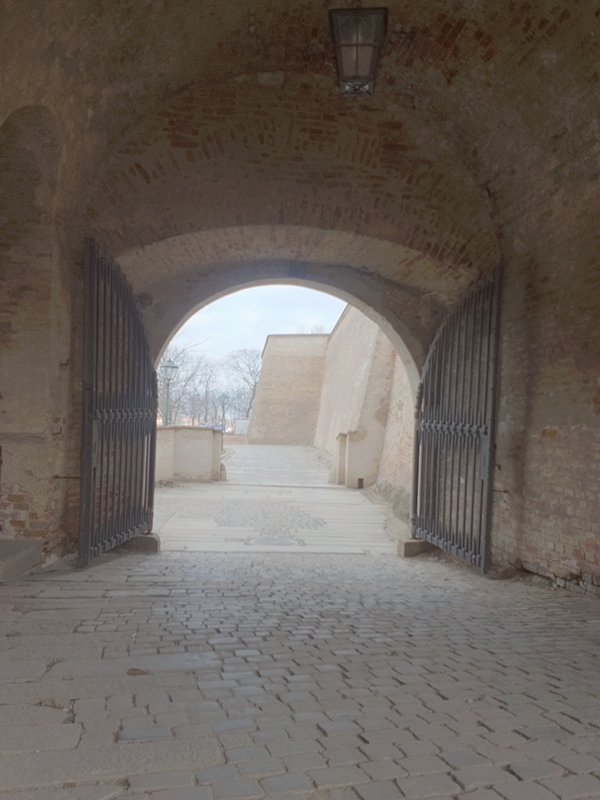
\includegraphics[width=\textwidth]{figures/tests/tmo/rein1}
  \end{subfigure}
  ~
  \begin{subfigure}{0.3\textwidth}
      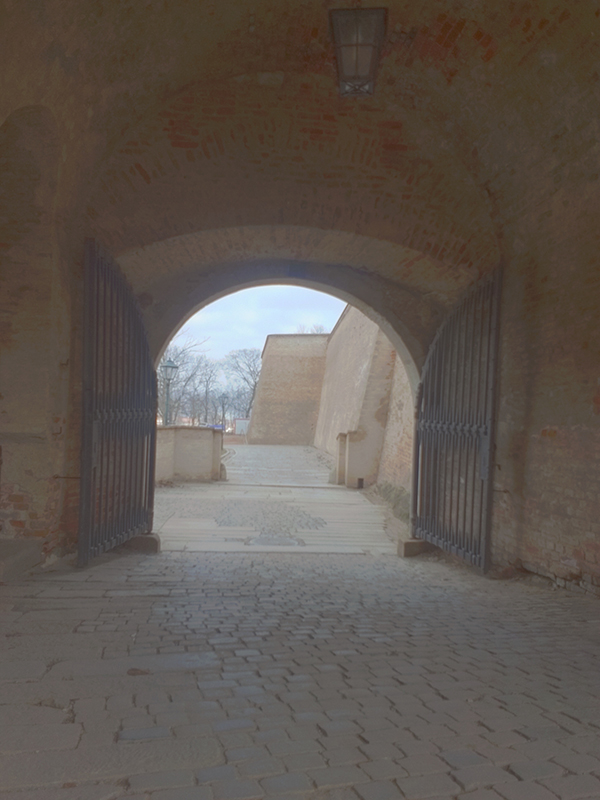
\includegraphics[width=\textwidth]{figures/tests/tmo/rein2}
  \end{subfigure}
  ~
  \begin{subfigure}{0.3\textwidth}
    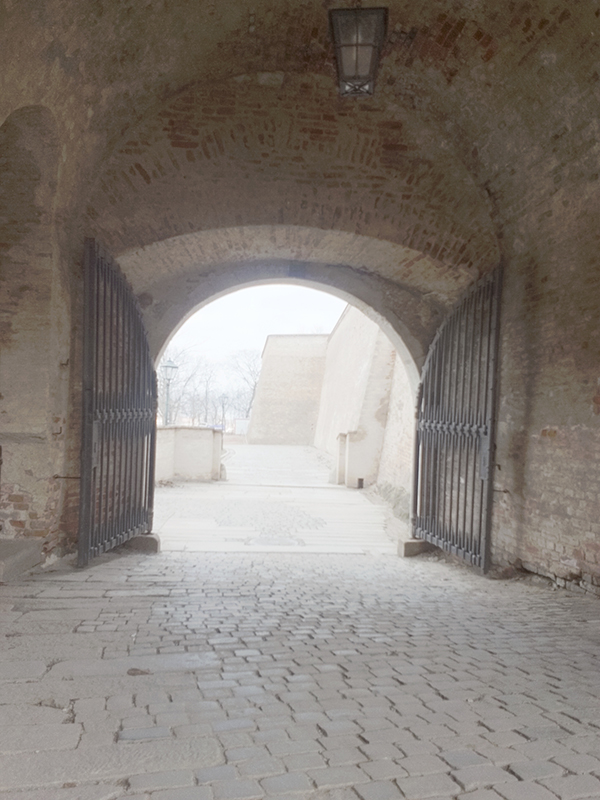
\includegraphics[width=\textwidth]{figures/tests/tmo/rein4}
  \end{subfigure}
  \caption{Výsledky mapovania tónov Reinhardovým operátorom}
  \label{fig:reinhards}
\end{figure}

Operátor \texttt{Drago} dokáže scénu s vysokým dynamickým rozsahom spracovať o niečo lepšie.
Jedinou užívateľom definovateľnou hodnotou je hodnota skreslenia (bias). Menšie hodnoty vytvárajú výrazne svetlejšie
snímky. Pri hodnotách, ktoré sa blížia minimu rozsahu nastáva na svetlých častiach nežiadúci stav - inverzia tónov,
zobrazená na treťom obrázku \ref{fig:dragos}.

\begin{figure}[h!]
  \centering
  \begin{subfigure}{0.3\textwidth}
      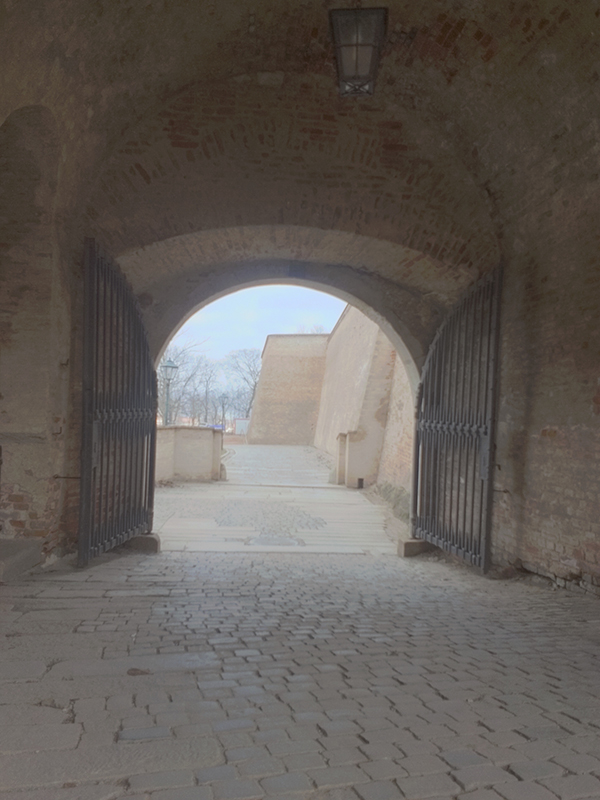
\includegraphics[width=\textwidth]{figures/tests/tmo/drag1}
  \end{subfigure}
  ~
  \begin{subfigure}{0.3\textwidth}
      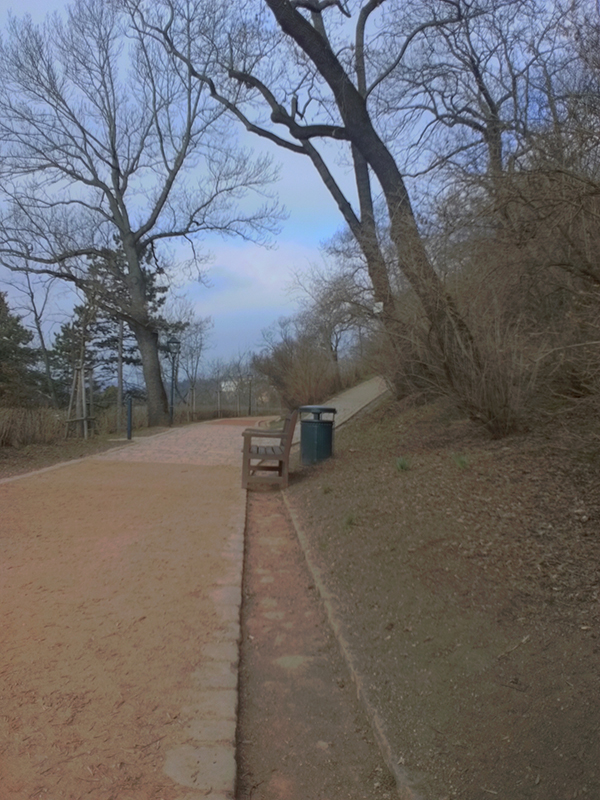
\includegraphics[width=\textwidth]{figures/tests/tmo/drag3}
  \end{subfigure}
  ~
  \begin{subfigure}{0.3\textwidth}
      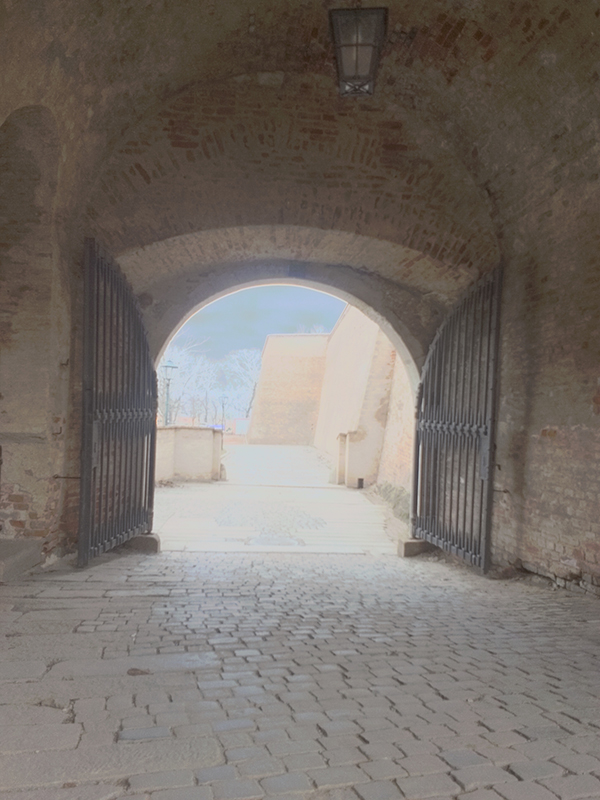
\includegraphics[width=\textwidth]{figures/tests/tmo/drag2}
  \end{subfigure}
  \caption{Výsledky mapovania tónov operátorom Drago}
  \label{fig:dragos}
\end{figure}

Lokálny operátor \texttt{Mantiuk} neponúka množstvo možností definovania vstupných parametrov. Aj preto možno užívateľ
nedokáže nájsť vhodné hodnoty nastavení, ktoré pre svoju scénu s vysokým dynamickým rozsahom potrebuje (obr.
\ref{fig:mantiuks}).

\begin{figure}[h!]
  \centering
  \begin{subfigure}{0.3\textwidth}
      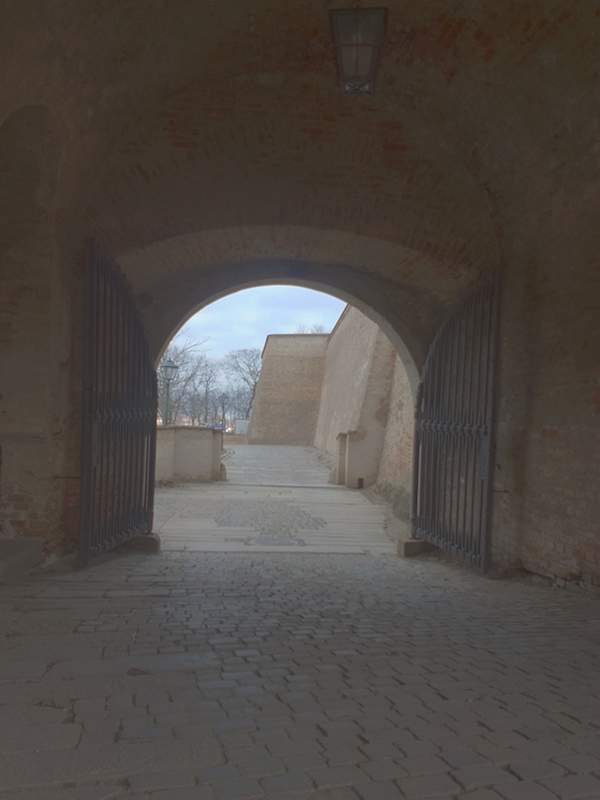
\includegraphics[width=\textwidth]{figures/tests/tmo/man3}
  \end{subfigure}
  ~
  \begin{subfigure}{0.3\textwidth}
      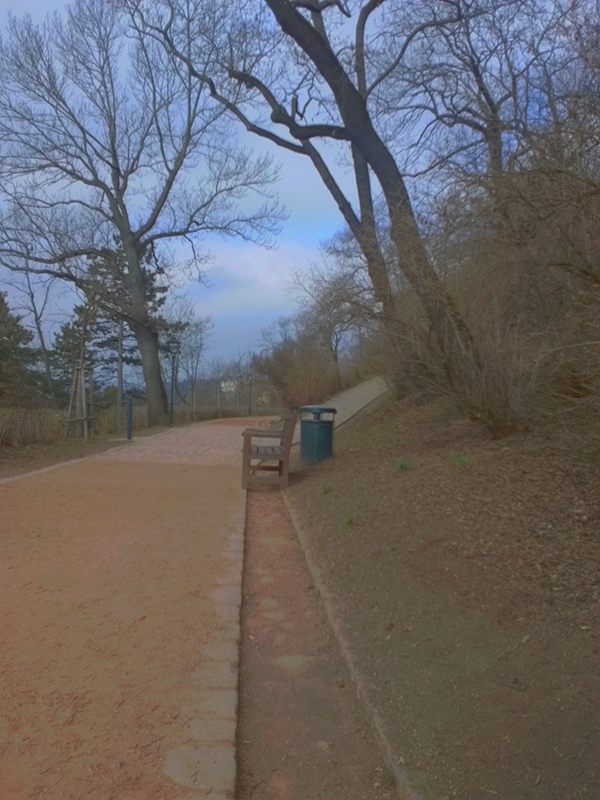
\includegraphics[width=\textwidth]{figures/tests/tmo/man4}
  \end{subfigure}
  \caption{Výsledky mapovania tónov operátorom Mantiuk}
  \label{fig:mantiuks}
\end{figure}

Najlepšie výsledky ponúka užívateľovi lokálny operátor \texttt{Durand}. Zo všetkých operátorov ponúka užívateľovi
najviac možností editovania vstupných parametrov. Pomocou nastavenia kontrastu môže užívateľ dobre definovať pomer výsledných
hodnôt jasu a tak vytvárať obrazy verne zobrazujúce scénu alebo obrazy s umeleckým efektom (obr. \ref{fig:durandUsage}).
Nastavovaním hodnôt bilaterálneho filtra \texttt{sigma color} a \texttt{sigma space} užívateľ zdôrazňuje detaily scény.

\begin{figure}[h!]
  \centering
  \begin{subfigure}{0.3\textwidth}
      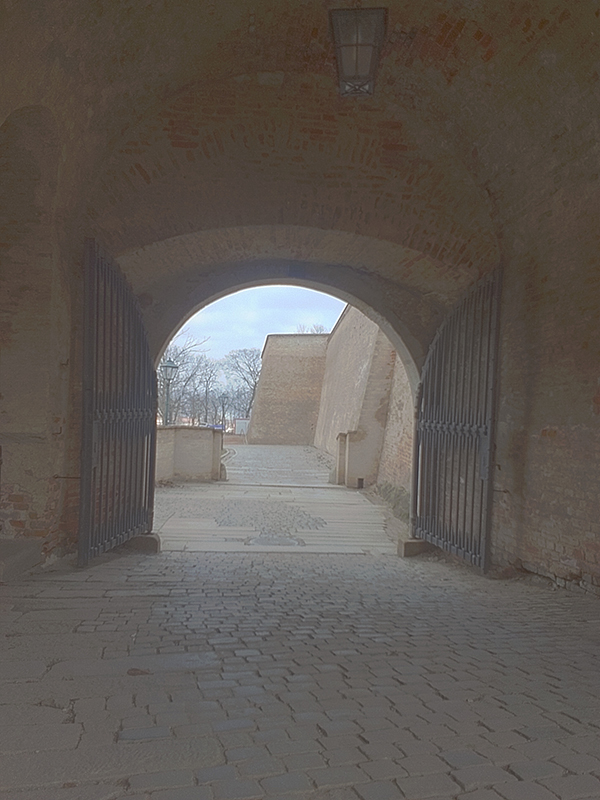
\includegraphics[width=\textwidth]{figures/tests/tmo/dur2}
  \end{subfigure}
  ~
  \begin{subfigure}{0.3\textwidth}
      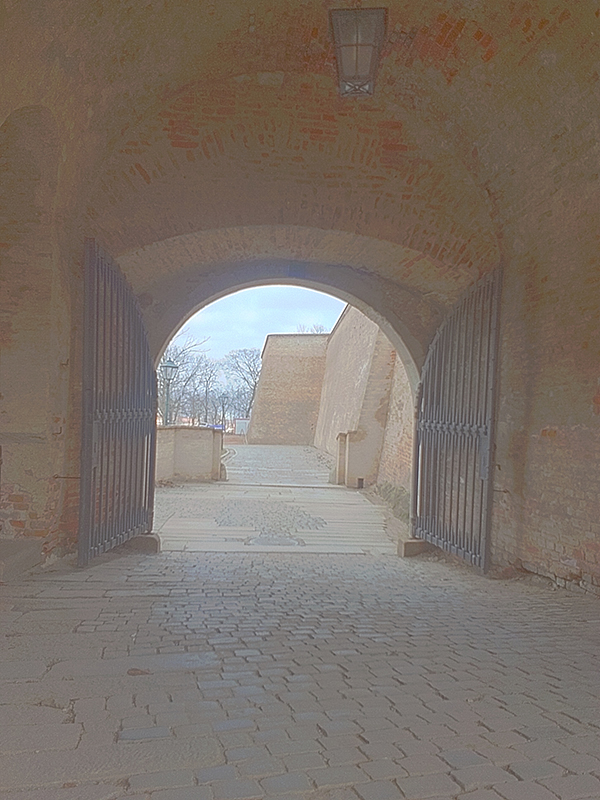
\includegraphics[width=\textwidth]{figures/tests/tmo/dur3}
  \end{subfigure}
  ~
  \begin{subfigure}{0.3\textwidth}
      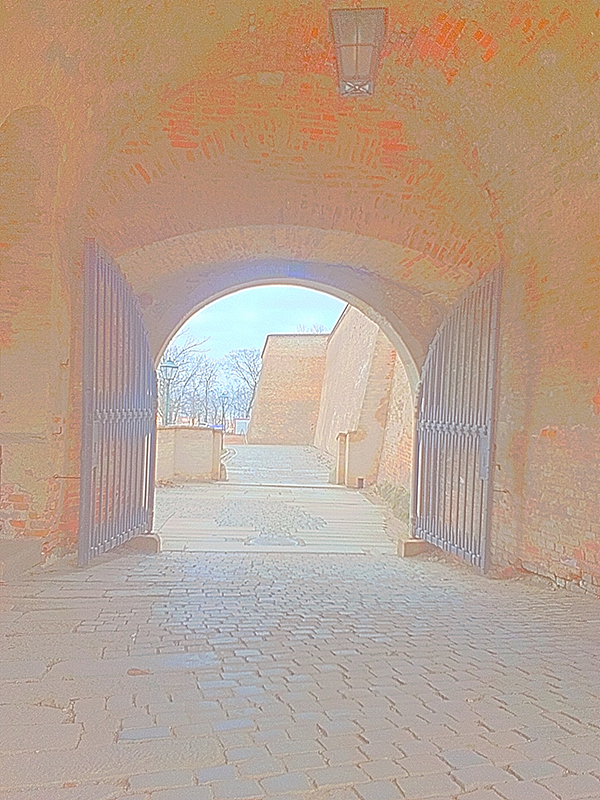
\includegraphics[width=\textwidth]{figures/tests/tmo/dur5}
  \end{subfigure}
  \caption{Výsledky mapovania tónov operátorom Durand}
  \label{fig:durands}
\end{figure}

\begin{figure}[h!]
  \centering
  \begin{subfigure}{0.3\textwidth}
      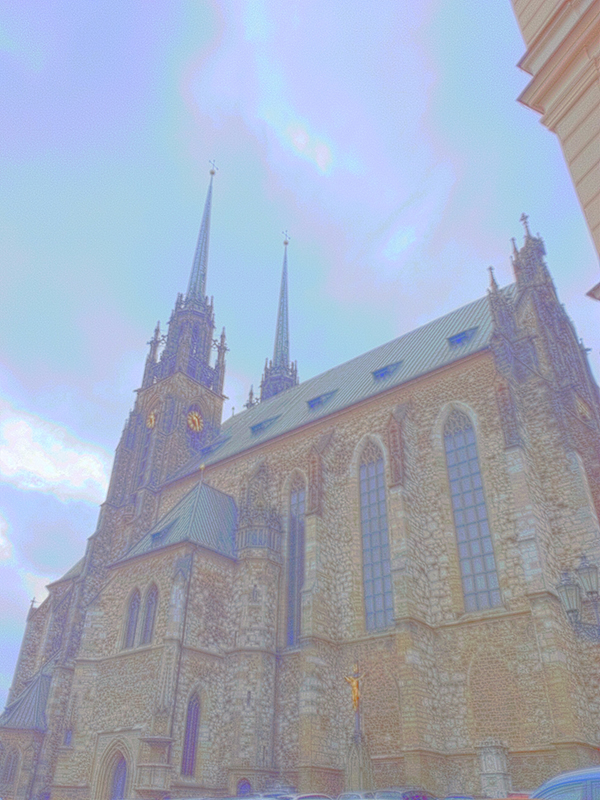
\includegraphics[width=\textwidth]{figures/tests/tmo/durSpace1}
      \caption{Vyhladenie}
  \end{subfigure}
  ~
  \begin{subfigure}{0.3\textwidth}
      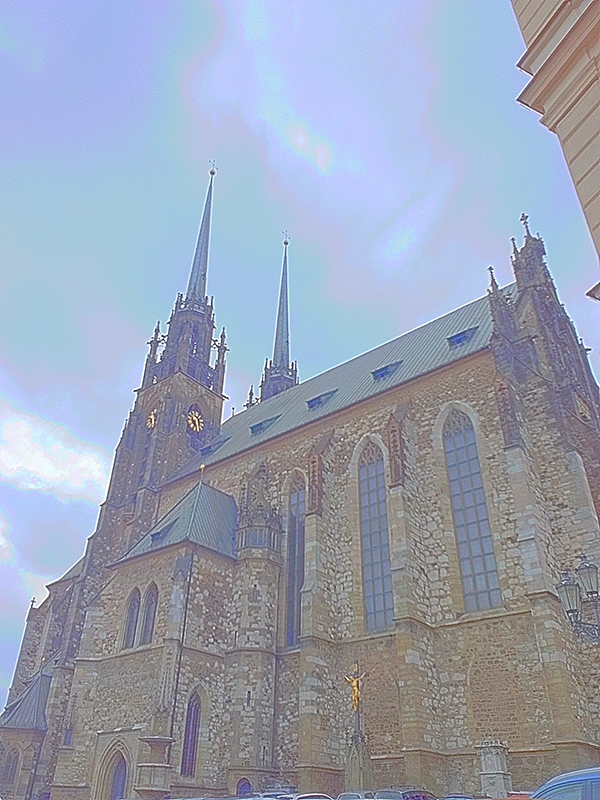
\includegraphics[width=\textwidth]{figures/tests/tmo/durSpace2}
      \caption{Zvýraznenie detailov}
  \end{subfigure}
  ~
  \begin{subfigure}{0.3\textwidth}
      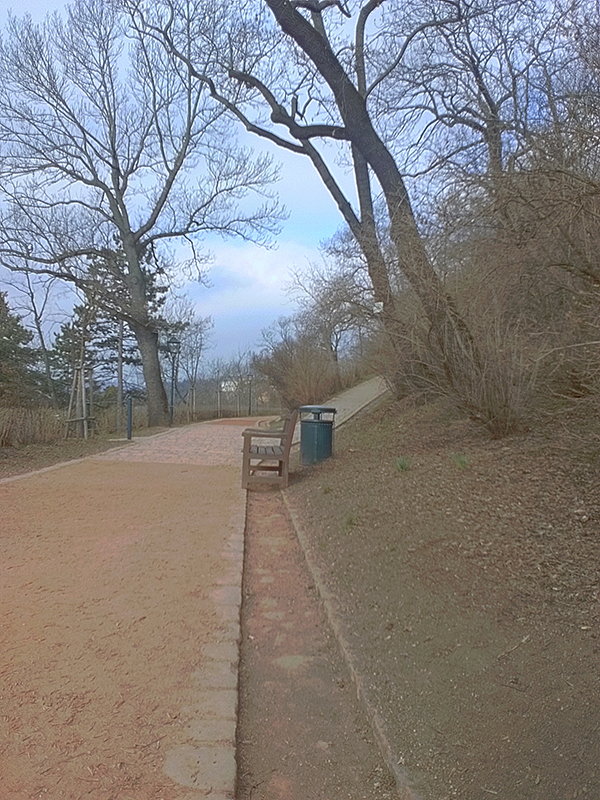
\includegraphics[width=\textwidth]{figures/tests/tmo/durVerna2}
      \caption{Verné zobrazenie scény}
  \end{subfigure}
  \caption{Obrazy verne zobrazujúce scénu ale aj umelecké efekty}
  \label{fig:durandUsage}
\end{figure}

Pri vysokých hodnotách \texttt{sigma color} a zároveň \texttt{sigma space} nastáva na hrane svetlej a tmavej oblasti halo efekt.
Operátor zahrnie pri výpočte blízko takejto hrany aj druhú stranu prechodu a zvýši kontrast naprieč hranou. Halo efekt je v
profesionálnej fotografii považovaný za chybu pri zobrazovaní reálnej scény. Veľa amatérskych fotografov však považuje toto
skreslenie ako súčasť umeleckého efektu fotografie.

\begin{figure}[h!]
  \centering
  \begin{subfigure}{0.3\textwidth}
      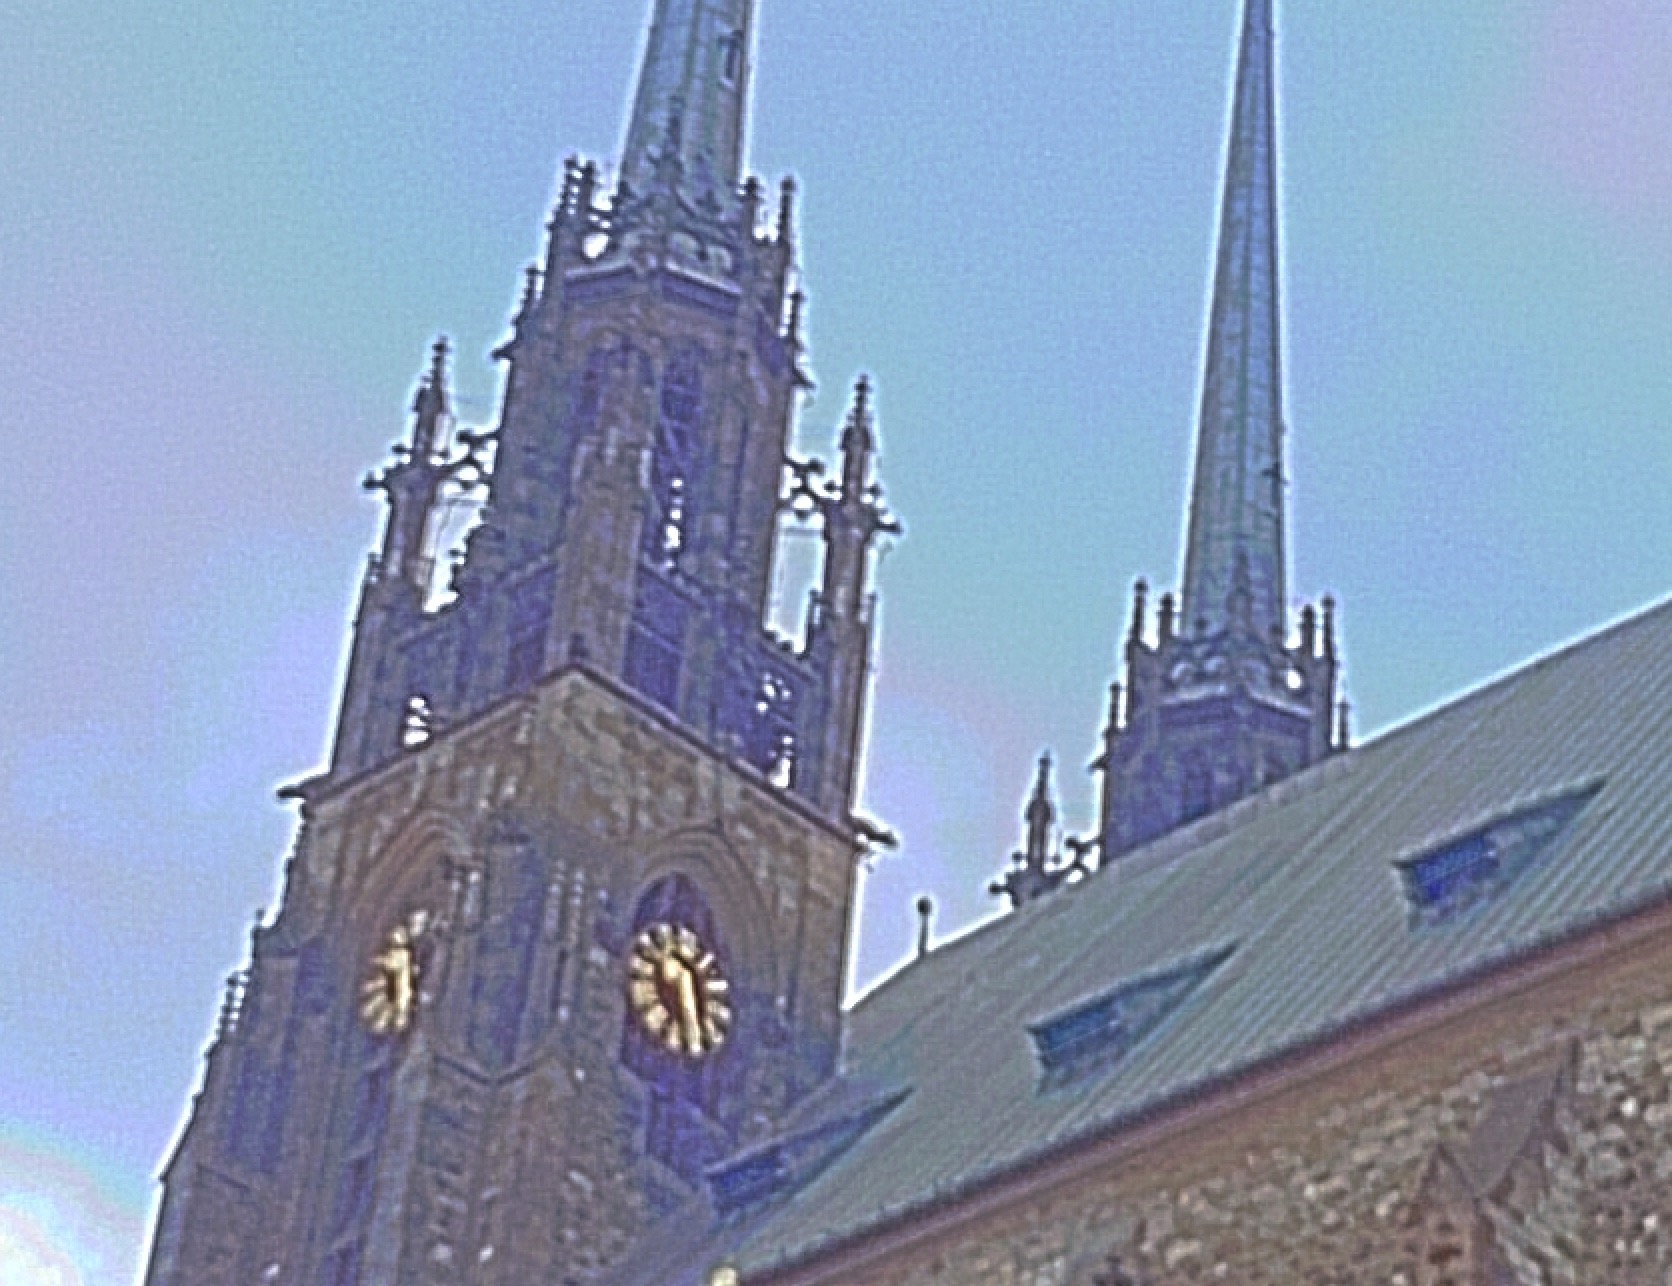
\includegraphics[width=\textwidth]{figures/tests/tmo/durHalo1}
  \end{subfigure}
  ~
  \begin{subfigure}{0.3\textwidth}
      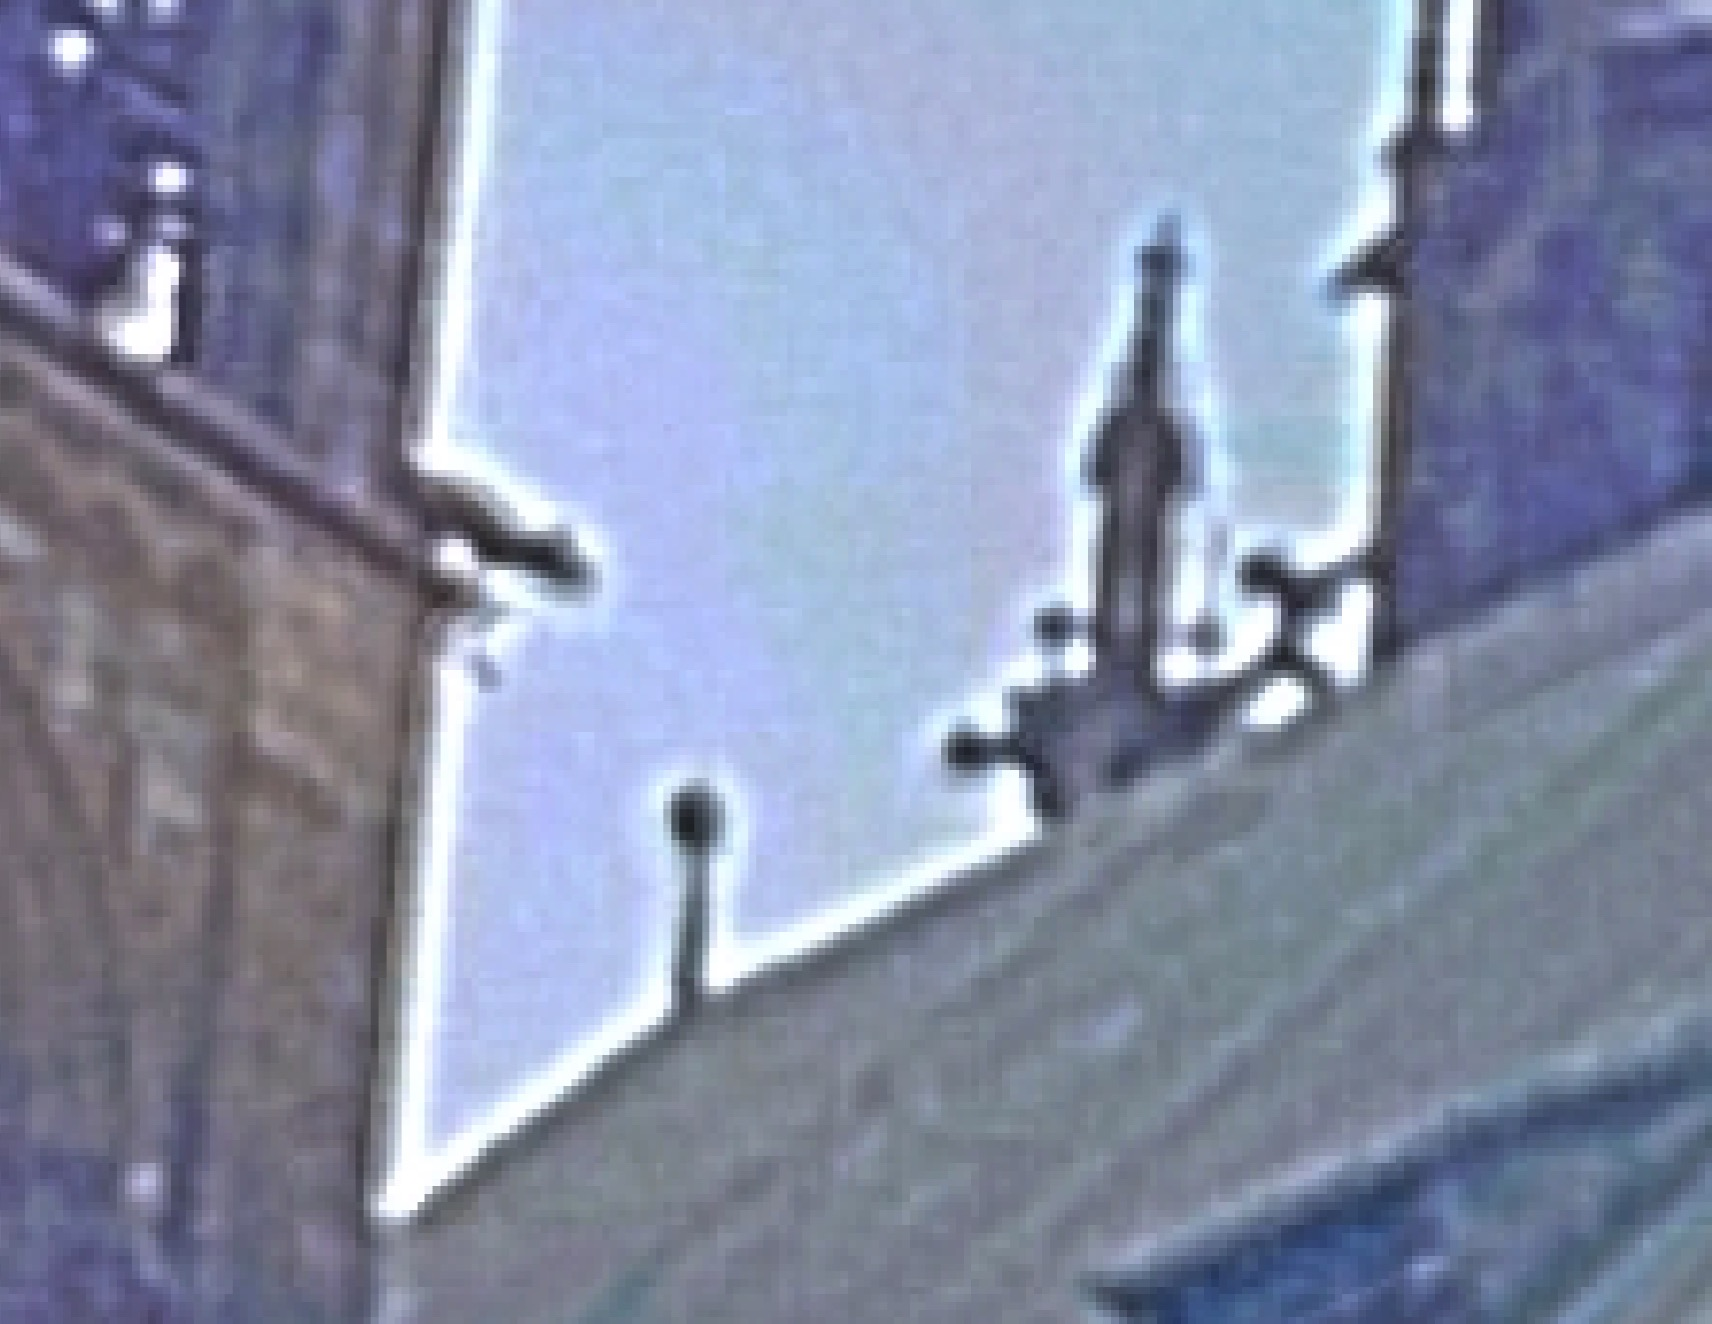
\includegraphics[width=\textwidth]{figures/tests/tmo/durHalo2}
  \end{subfigure}
  \caption{Halo efekt spôsobený ostrým prechodom medzi zreteľne svetlou a tmavou oblasťou}
  \label{fig:durandHalo}
\end{figure}
